\documentclass[dvipdfmx,aspectratio=169]{beamer}
\usepackage{amsmath}
\usepackage{booktabs}
\usepackage{pxjahyper}
\usepackage{tikz}
\usetikzlibrary{arrows.meta,positioning,backgrounds}

\usetheme{Madrid}
\usecolortheme{default}
\setbeamertemplate{navigation symbols}{}

\title[ABC462 C]{AtCoder ABC462 -- C\\\small Not Covered Points の解説}
\author{}
\date[CodeQUEEN 2026]{CodeQUEEN 2026 -qual- / 300 点}

% よく使う色
\definecolor{ok}{RGB}{0,140,70}
\definecolor{ng}{RGB}{200,30,30}

\begin{document}

\begin{frame}
  \titlepage
\end{frame}

%====================================================================
\begin{frame}{問題の概要}
  \begin{itemize}
    \item $2$ 次元平面に点 $1,2,\ldots,N$ があり，点 $i$ の座標は $(X_i, Y_i)$．
    \item $X, Y$ はそれぞれ $(1,2,\ldots,N)$ の\textbf{順列}（同じ座標値は重複しない）．
    \item 各 $i$ について，左下 $(0,0)$・右上 $(X_i,Y_i)$ の軸平行な長方形を考える．
    \item その長方形の\textbf{内部（辺上を含まない）}に，$N$ 個の点をどれも含まない
      ような $i$ の\textbf{個数}を求める．
  \end{itemize}

  \vspace{0.8em}
  \textbf{制約}: $1 \le N \le 3\times 10^5$,\quad $1 \le X_i,Y_i \le N$,\quad
  $X,Y$ は順列．

  \vspace{0.4em}
  \begin{block}{計算量の目標}
    全探索 $O(N^2)$ は TLE．\textbf{$O(N\log N)$} を狙う．
  \end{block}
\end{frame}

%====================================================================
\begin{frame}{言い換え：効くのは「真の左下」だけ}
  点 $j$ が点 $i$ の長方形の\textbf{内部}に入る条件は，辺上を除くので
  \[
    \boxed{\,X_j < X_i \ \text{かつ}\ Y_j < Y_i\,}
    \quad(\text{$j$ は $i$ の真の左下にいる})
  \]

  \vspace{0.3em}
  \begin{columns}
    \begin{column}{0.52\textwidth}
      よって
      \begin{itemize}
        \item 点 $i$ が条件を満たす（\textbf{Not Covered}）
        \item $\Longleftrightarrow$ 自分より\textbf{真の左下に点が $1$ つも無い}
      \end{itemize}
      \vspace{0.5em}
      長方形そのものを考える必要はなく，
      「\textbf{左下に点があるか}」の判定問題に帰着する．
    \end{column}
    \begin{column}{0.46\textwidth}
      \centering
      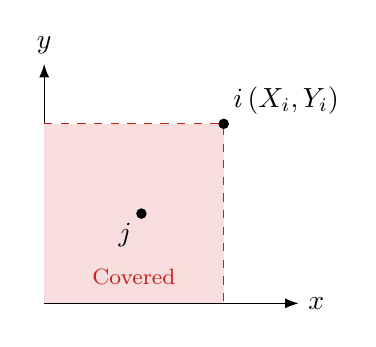
\begin{tikzpicture}[scale=0.95]
        % 軸
        \draw[-{Latex}] (0,0) -- (3.4,0) node[right]{$x$};
        \draw[-{Latex}] (0,0) -- (0,3.2) node[above]{$y$};
        % 点 i
        \coordinate (I) at (2.4,2.4);
        % 左下の覆い領域
        \fill[ng!15] (0,0) rectangle (2.4,2.4);
        \draw[ng,dashed] (0,2.4) -- (2.4,2.4) -- (2.4,0);
        % 点 j (内部)
        \fill (1.3,1.2) circle (2pt) node[below left]{$j$};
        % 点 i
        \fill (I) circle (2pt) node[above right]{$i\,(X_i,Y_i)$};
        \node[ng] at (1.2,0.35) {\footnotesize Covered};
      \end{tikzpicture}
    \end{column}
  \end{columns}
\end{frame}

%====================================================================
\begin{frame}{解法：$X$ 昇順ソート $+$ $Y$ の prefix 最小}
  \begin{columns}
    \begin{column}{0.5\textwidth}
      \textbf{Step 1.} 点を $X$ の\textbf{昇順}に走査．\\
      $\Rightarrow$「自分より左（$X$ が小）」の点は走査済み．

      \vspace{0.6em}
      \textbf{Step 2.} それまでに見た $Y$ の最小値 $\mathrm{minY}$ だけ持てば判定可能：
      \begin{itemize}
        \item $\mathrm{minY} < Y_i$\ \ $\Rightarrow$ 左下に点あり（\textcolor{ng}{Covered}）
        \item $Y_i < \mathrm{minY}$\ \ $\Rightarrow$ 左下に点なし
          （\textcolor{ok}{Not Covered}：\,$ans{+}{+}$, $\mathrm{minY}$ 更新）
      \end{itemize}
      \vspace{0.5em}
      答え $=$「$X$ 昇順での $Y$ の\textbf{prefix minimum 更新回数}」．
    \end{column}
    \begin{column}{0.5\textwidth}
      \centering
      \begin{tikzpicture}[scale=0.9]
        \draw[-{Latex}] (0,0) -- (4.2,0) node[right]{\footnotesize $X$};
        \draw[-{Latex}] (0,0) -- (0,3.6) node[above]{\footnotesize $Y$};
        % 階段（min Y は非増加）
        \draw[very thick, ok]
          (0,3.2) -- (1,3.2) -- (1,2.1) -- (2,2.1)
          -- (2,1.2) -- (3,1.2) -- (3,0.6) -- (4,0.6);
        % 更新点（prefix minima）
        \fill (1,3.2) circle (2pt);
        \fill (2,2.1) circle (2pt);
        \fill (3,1.2) circle (2pt);
        \fill (4,0.6) circle (2pt);
        % 覆われる点（階段の上側）
        \fill[gray] (1.6,2.8) circle (1.6pt);
        \fill[gray] (2.7,1.9) circle (1.6pt);
        \fill[gray] (3.4,1.0) circle (1.6pt);
        \node[ok] at (3.0,3.0) {\footnotesize 階段＝更新点};
        \node[gray] at (3.3,2.4) {\footnotesize 上側＝Covered};
      \end{tikzpicture}
    \end{column}
  \end{columns}
\end{frame}

%====================================================================
\begin{frame}{サンプル 1 を手で動かす}
  入力 $N=3$，点 $(2,1),(1,3),(3,2)$\quad
  $\Rightarrow$\quad $X$ 昇順ソート：$(1,3),(2,1),(3,2)$

  \vspace{0.6em}
  \begin{center}
  \begin{tabular}{ccccll}
    \toprule
    順 & 点 $(X,Y)$ & 直前 $\mathrm{minY}$ & $Y<\mathrm{minY}$? & 判定 & $ans$\\
    \midrule
    1 & $(1,3)$ & $\infty$ & yes & \textcolor{ok}{Not Covered} & 1\\
    2 & $(2,1)$ & $3$ & yes & \textcolor{ok}{Not Covered} & 2\\
    3 & $(3,2)$ & $1$ & no  & \textcolor{ng}{Covered} & 2\\
    \bottomrule
  \end{tabular}
  \end{center}

  \vspace{0.6em}
  \begin{alertblock}{答え：2}
    $i=3$ の長方形 $(0,0)$--$(3,2)$ は内部に点 $1$ $(2,1)$ を含むので不適．
  \end{alertblock}
\end{frame}

%====================================================================
\begin{frame}[fragile]{実装（Python，$O(N\log N)$）}
\begin{verbatim}
import sys
input = sys.stdin.readline

n = int(input())
pts = [tuple(map(int, input().split())) for _ in range(n)]
pts.sort(key=lambda p: p[0])          # X 昇順

ans = 0
min_y = float("inf")
for _, y in pts:
    if y < min_y:                     # 真の左下に点が無い
        ans += 1
        min_y = y
print(ans)
\end{verbatim}
  \vspace{-0.3em}
  ソートが支配的で全体 $O(N\log N)$．判定自体は $1$ パス $O(N)$．
\end{frame}

%====================================================================
\begin{frame}{注意：正しい「双対」と，メモの落とし穴}
  \begin{block}{正しい双対（同じ答えになる）}
    「真の左下に点が無いか」は，\textbf{$X$ と $Y$ の役割を入れ替えても}
    よい：$Y$ 昇順ソート $+$ $X$ の prefix 最小でも\textbf{同じ答え}．
  \end{block}

  \begin{alertblock}{落とし穴：「右上に点があるか」は\underline{別問題}}
    手書きメモには覆う条件を $X_i<X_j \wedge Y_i<Y_j$（自分より\textbf{右上}に点）
    と書いた箇所があるが，これは
    「右上に点が無い点（Pareto 最大点）の数」を数えることになり\textbf{別物}．
  \end{alertblock}

  \footnotesize 反例：$(1,1),(2,3),(3,2)$ では
  \emph{正答 $=1$} だが，右上版は $2$ を返す
  （$N=5$ の全 $120$ 順列のうち $74$ 通りでズレる）．
  \normalsize

  \vspace{0.4em}
  \textbf{要点}：この問題で効くのは「\textbf{左下}に点があるか」のみ．
  典型は ABC091 C「2D Plane 2N Points」と同系統の「ソートして貪欲」．
\end{frame}

\end{document}
